\chapter{\LTLfToDFA}\label{ch:ltlf2dfa}
In this chapter we will present \href{https://github.com/Francesco17/LTLf2DFA}{\LTLfToDFA}, a software package  written in Python. 

\section{Introduction}
\LTLfToDFA is a Python tool that processes a given \LTLf formula (with past and future operators) and generates the corresponding minimized \DFA using \MONA\citep{mona1998}.
The main features provided by the library are:
\begin{itemize}
\item parsing an \LTLf formula with past or future operators;
\item translation of an \LTLf formula to \MONA program;
\item conversion of an \LTLf formula to \DFA automaton.
\end{itemize}
\LTLfToDFA can be used with Python>=3.6 and has the following dependencies:
\begin{itemize}
\item \href{http://www.dabeaz.com/ply/ply.html}{PLY}, a pure-Python implementation of the popular compiler construction tools \href{http://dinosaur.compilertools.net/}{Lex and Yacc}. It has been employed for parsing the input \LTLf formula;
\item \href{http://www.brics.dk/mona/}{\MONA}, a C++ tool that translates formulas to \DFA. It has been used for the generation of the \DFA;
\item \href{https://pypi.org/project/dotpy/}{Dotpy}, a Python library able to parse and modify \texttt{.dot} files. It has been utilized for post-processing the \MONA output.
\end{itemize}
The package is available to download on \href{https://pypi.org/project/ltlf2dfa/}{PyPI} and you can install it typing in the terminal:
\begin{lstlisting}[language=bash]
pip install ltlf2dfa
\end{lstlisting}
All the code is available online on GitHub\footnote{https://github.com/Francesco17/LTLf2DFA}, it is open source and it is released under the \href{https://github.com/Francesco17/LTLf2DFA/blob/master/LICENSE}{MIT License}.
Moreover, \LTLfToDFA can also be tried online at \href{ltlf2dfa.diag.uniroma1.it}{ltlf2dfa.diag.uniroma1.it}.
\section{Package Structure}
The structure of the \LTLfToDFA package is quite simple. It consists of a main folder called \texttt{ltlf2dfa/} which hosts the most important library's modules:
\begin{itemize}
\item \texttt{Lexer.py}, where the Lexer class is defined;
\item \texttt{Parser.py}, where the Parser class is defined;
\item \texttt{Translator.py}, where the main APIs for the translation are defined;
\item \texttt{DotHandler.py}, where we the \MONA output is post-processed.
\end{itemize}
In the following paragraphs we will explore each module in detail.
\subsection{Lexer.py}
In the \texttt{Lexer.py} module we can find the declaration of the \texttt{MyLexer} class which is in charge of handling the input string and tokenize it. Indeed, it implements a tokenizer that splits the input string into declared individual tokens.
To our extent, we have defined the class as in Listing \ref{code:ltlf2dfa-lexer}
\begin{lstlisting}[language=Python, style=Python, label={code:ltlf2dfa-lexer}, caption={\texttt{Lexer.py} module}]
import ply.lex as lex

class MyLexer(object):

    reserved = {
        'true':     'TRUE',
        'false':    'FALSE',
        'X':        'NEXT',
        'U':        'UNTIL',
        'E':        'EVENTUALLY',
        'G':        'GLOBALLY',
        'Y':        'PASTNEXT', #PREVIOUS
        'S':        'PASTUNTIL', #SINCE
        'O':        'PASTEVENTUALLY', #ONCE
        'H':        'PASTGLOBALLY'
    }
    # List of token names.   This is always required
    tokens = (
        'TERM',
        'NOT',
        'AND',
        'OR',
        'IMPLIES',
        'DIMPLIES',
        'LPAR',
        'RPAR'
    ) + tuple(reserved.values())

    # Regular expression rules for simple tokens
    t_TRUE = r'T'
    t_FALSE = r'F'
    t_AND = r'\&'
    t_OR = r'\|'
    t_IMPLIES = r'\->'
    t_DIMPLIES = r'\<->'
    t_NOT = r'\~'
    t_LPAR = r'\('
    t_RPAR = r'\)'
    # FUTURE OPERATORS
    t_NEXT = r'X'
    t_UNTIL = r'U'
    t_EVENTUALLY = r'E'
    t_GLOBALLY = r'G'
    # PAST OPERATOR
    t_PASTNEXT = r'Y'
    t_PASTUNTIL = r'S'
    t_PASTEVENTUALLY = r'O'
    t_PASTGLOBALLY = r'H'

    t_ignore = r' '+'\n'

    def t_TERM(self, t):
        r'[a-z]+'
        t.type = MyLexer.reserved.get(t.value, 'TERM')
        return t  # Check for reserved words

    def t_error(self, t):
        print("Illegal character '%s' in the input formula" % t.value[0])
        t.lexer.skip(1)

    # Build the lexer
    def build(self,**kwargs):
        self.lexer = lex.lex(module=self, **kwargs)
\end{lstlisting}
Firstly, we have defined the reserved words within a dictionary so to match each reserved word with its identifier.
Secondly, we have defined the tokens list with all possible tokens that can be produced by the lexer. The tokens list is always required for the implementation of a lexer.
Then, each token has to be specified by writing a regular expression rule. If the token is simple it can be specified using only a string. Otherwise, for non trivial tokens we have to write the regular expression in a class method as for our token \texttt{TERM}. In that case, defining the token rule as a method is useful also when we would like to perform other actions. After that, we have a method to handle unrecognized tokens and, finally, we can build the lexer.
\subsection{Parser.py}
In the \texttt{Parser.py} module we can find the declaration of \texttt{MyParser} class which implements the parsing component of \texttt{PLY}. The \texttt{MyParser} class operates after the Lexer has split the input string into known tokens. The main feature of the parser is to interpret and build the appropriate data structure for the given input. To this extent, the most important aspect of a parser is the definition of the \textit{syntax}, usually specified in terms of a BNF grammar, that should be unambiguous. Furthermore, Yacc, the parsing component of \texttt{PLY}, implements a parsing technique known as LR-parsing or shift-reduce parsing. In particular, this parsing technique works on a bottom up fashion that tries to recognize the right-hand-side of various grammar rules. Whenever a valid right-hand-side is found in the input, the appropriate action code is triggered and the grammar symbols are replaced by the grammar symbol on the left-hand-side and so on until there is no more rule to apply. The parser implementation is shown in Listing \ref{code:ltlf2dfa-parser}
\begin{lstlisting}[language=Python, style=Python, label={code:ltlf2dfa-parser}, caption={\texttt{Parser.py} module}]
import ply.yacc as yacc
from ltlf2dfa.Lexer import MyLexer

class MyParser(object):

    def __init__(self):
        self.lexer = MyLexer()
        self.lexer.build()
        self.tokens = self.lexer.tokens
        self.parser = yacc.yacc(module=self)
        self.precedence = (

            ('nonassoc', 'LPAR', 'RPAR'),
            ('left', 'AND', 'OR', 'IMPLIES', 'DIMPLIES', 'UNTIL', \
             'PASTUNTIL'),
            ('right', 'NEXT', 'EVENTUALLY', 'GLOBALLY', \
            'PASTNEXT', 'PASTEVENTUALLY', 'PASTGLOBALLY'),
            ('right', 'NOT')
        )

    def __call__(self, s, **kwargs):
        return self.parser.parse(s, lexer=self.lexer.lexer)

    def p_formula(self, p):
        '''
        formula : formula AND formula
                | formula OR formula
                | formula IMPLIES formula
                | formula DIMPLIES formula
                | formula UNTIL formula
                | formula PASTUNTIL formula
                | NEXT formula
                | EVENTUALLY formula
                | GLOBALLY formula
                | PASTNEXT formula
                | PASTEVENTUALLY formula
                | PASTGLOBALLY formula
                | NOT formula
                | TRUE
                | FALSE
                | TERM
        '''

        if len(p) == 2: p[0] = p[1]
        elif len(p) == 3:
            if p[1] == 'E': # E(a) == true UNITL A
                p[0] = ('U','T', p[2])
            elif p[1] == 'G': # G(a) == not(eventually (not A))
                p[0] = ('~',('U', 'T', ('~',p[2])))
            elif p[1] == 'O': # O(a) = true SINCE A
                p[0] = ('S','T', p[2])
            elif p[1] == 'H': # H(a) == not(pasteventually(not A))
                p[0] = ('~',('S', 'T', ('~',p[2])))
            else:
                p[0] = (p[1], p[2])
        elif len(p) == 4:
            if p[2] == '->':
                p[0] = ('|', ('~', p[1]), p[3])
            elif p[2] == '<->':
                p[0] = ('&', ('|', ('~', p[1]), p[3]), ('|', ('~', p[3]),\
                p[1]))
            else:
                p[0] = (p[2],p[1],p[3])
        else: raise ValueError


    def p_expr_group(self, p):
        '''
        formula : LPAR formula RPAR
        '''
        p[0] = p[2]

    def p_error(self, p):
        raise ValueError("Syntax error in input! %s" %str(p))
\end{lstlisting}
As we can see, as soon as the parser is instantiated it builds the lexer, gets the tokens and defines their precedence if needed. Then, we have defined methods of the \texttt{MyParser} class that are in charge of constructing the syntax tree structure from tokens found by the lexer in the input string. In our case, we have chosen to use as data structure a tuple of tuples as it is the one of the simplest data structure in Python. In general, a tuple of tuples represents a tree where each node represents an item in the formula.

For instance, the \LTLf formula $\varphi= G(a \rightarrow X b)$ is represented as $('\thicksim', ('U', 'T', ('\thicksim',('|', ('\thicksim', 'a'), ('X', 'b')))))$ as depicted in Figure \ref{fig:formula-syntax-tree}.
\begin{figure}[h]
	\centering
	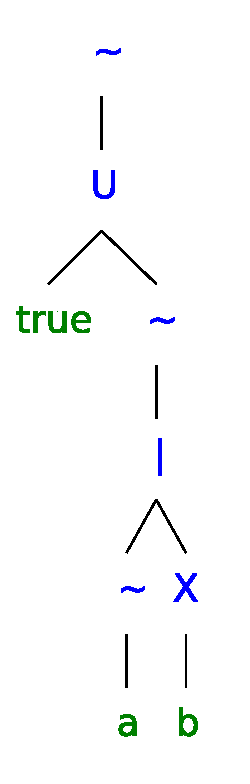
\includegraphics[height=15em, width=7.5em]{images/formula-syntax-tree}
	\caption{The syntax tree generated for the formula $"G(a \thicksim Xb)"$. Symbols are in green while operators are in blue.}
	\label{fig:formula-syntax-tree}
\end{figure}
Finally, as in the \texttt{MyLexer} class, we have to handle errors defining a specific method.

\LTLfToDFA can be used just for the parsing phase of an 	\LTLf formula as shown in Listing \ref{code:ltlf2dfa-only-parsing}.
\begin{lstlisting}[language=Python, style=Python, label={code:ltlf2dfa-only-parsing}, caption={How to use only the parsing phase of \LTLfToDFA.}]
from ltlf2dfa.Parser import MyParser

formula = "G(a->Xb)"
parser = MyParser()
parsed_formula = parser(formula)

print(parsed_formula) # syntax tree as tuple of tuples
\end{lstlisting}
\subsection{Translator.py}
The \texttt{Translator.py} module contains the majority of APIs that the \LTLfToDFA package exposes. Indeed, this module consists of a Translator class which concerns the core feature of the package: the translation of an \LTLf  formula into a \DFA. Since the package takes advantage of the \MONA tool for the formula conversion, the \texttt{Translator} class has to translate the given formula in the syntax recognized by \MONA, create the input program for \MONA and, finally, invoke \MONA to get back the resulting \DFA in the Graphviz\footnote{Graphviz is open source graph visualization software. For further details see \href{https://www.graphviz.org}{https://www.graphviz.org}} format. 
The main methods of the \texttt{Translator} class are:
\begin{itemize}
\item \texttt{translate()}, which starting from the formula syntax tree generated in the parsing phase translates it into a string using the syntax of \MONA\citep{monamanual2001};
\item \texttt{createMonafile(flag)}, which, as the name suggests, creates the program \textit{.mona} that will be given as input to \MONA. The flag parameter is going to be \texttt{True} of \texttt{False} whether we need to compute also \textsc{DECLARE}  assumptions or not;
\item \texttt{invoke\_mona()}, which invokes \MONA in order to obtain the \DFA.
\end{itemize}
\subsection{DotHandler.py}


















